\header{
    \section{De sur la mer} \label{de-sur-la-mer}
    %
    \insertComment{Chaque couplet est répété par le choeur}{}
}

\enluminure{2}{\href{https://www.dailymotion.com/video/x713v7#.UMTqxqyX11E}{D}}{e sur} la mer, savez-vous c'qu'il y a ? \bissimple
\\\\\\Y'a un bateau
\\Un bateau d'amour mes dames
\\Y'a un bateau
\\Un bateau d'amour joli.
\\\\Dans ce bateau savez c'qu'il y a \bissimple
\\\\Y'a un marin
\\Y'a un marin d'amour mes dames
\\Y'a un marin
\\Y'a un marin d'amour joli.
\\\\Sur ce marin, savez-vous c'qu'il y a ? \bissimple
\\\\Il y a t'une fiole
\\Y'a t'une fiole d'amour mes dames
\\Y'a t'une fiole
\\Y'a t'une fiole d'amour joli.
\\\\Et dans cette fiole, savez-vous c'qu'il y a ? \bissimple
\\\\Il y a d'la bière
\\Du whisky d'amour mes dames
\\Il y a d'la bière
\\Du whisky d'amour joli
\\\\Dans ce whisky, savez-vous c'qu'il y a ? \bissimple
\\\\Y a des femmes
\\Y a des femmes d'amour mes dames
\\Y a des femmes
\\Y a des femmes d'amour joli
\\\\Et dans ces femmes, savez-vous c'qu'il y a ? \bissimple
\\\\Y a d'l'ammour
\\Dans ces femmes d'amour mes dames
\\Y a d'l'ammour
\\Dans ces femmes d'amour joli
\\\\De sur la mer, savez-vous c'qu'il y a ? \bissimple
\\\\Y'a un bateau
\\Un bateau d'amour mes dames
\\Y'a un bateau
\\Un bateau d'amour joli.

\bigskip
\bigskip
\bigskip
\begin{center}
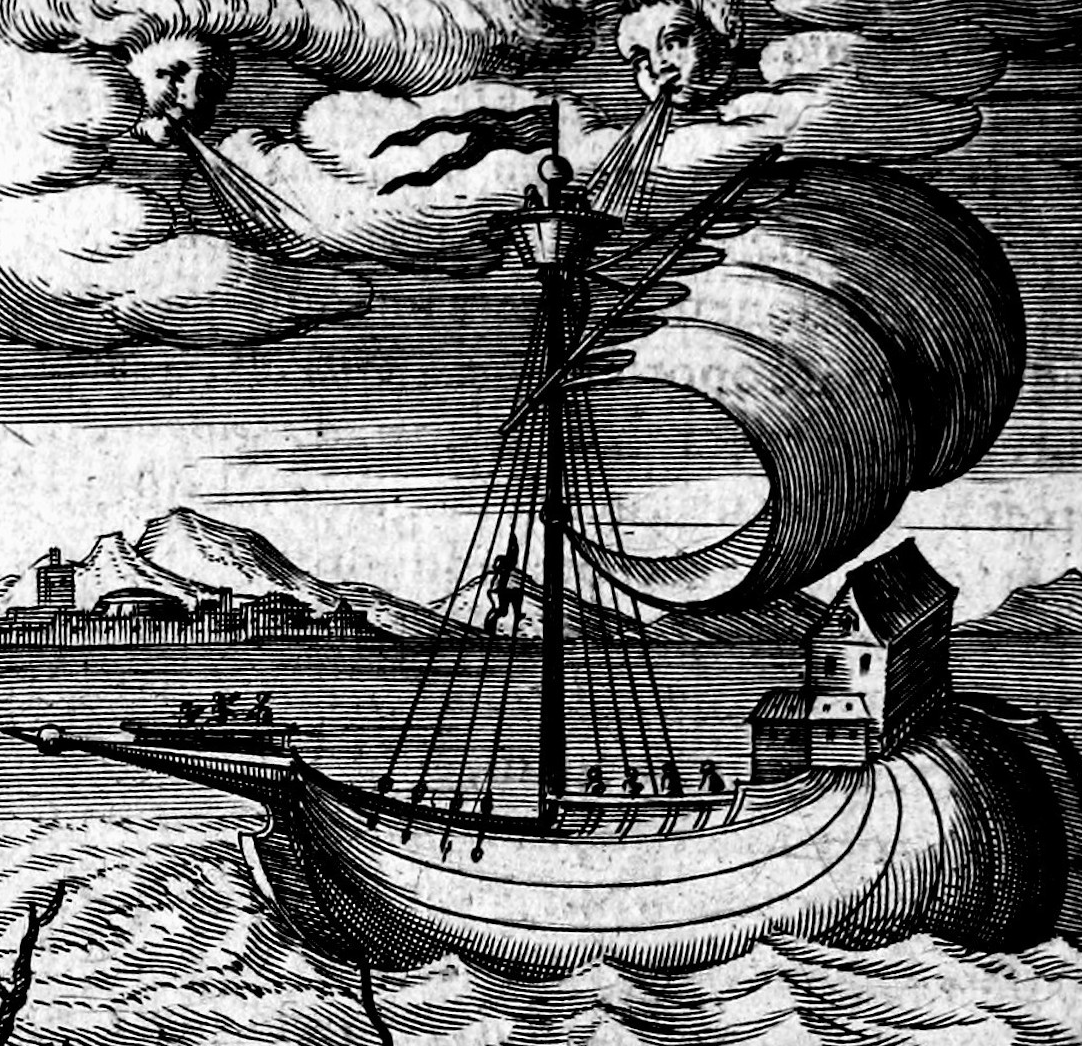
\includegraphics[width=1\textwidth]{images/brev27.png}
\end{center}

\breakpage